\chapter{Popis struktury adresáře}
\dirtree{%
.1 thesis-package\DTcomment{Kořenový adresář}.
.2 xchmel22\_ SP\DTcomment{Tato práce}.
.2 master-thesis\DTcomment{Zdrojové soubory pro tuto práci}.
.2 master-thesis-notebooks\DTcomment{Implementace v Jupyter notebook}.
.3 current\_ processing\_ methods\DTcomment{Současné metody}.
.3 image\_ series\_ preprocessing\DTcomment{Navržené metody}.
.4 dynamic\_ range\_ enhancement\DTcomment{Metody pro zvýšení dynamického rozsahu}.
.4 noise\_ reduction\DTcomment{Metody pro snížení šumu}.
}
Zdrojové soubory této práce a implementací v podobě Jupyter notebooků lze nalézt v repositářích:
\begin{itemize}
\item \url{https://github.com/petrchmelar/master-thesis}
\item \url{https://github.com/petrchmelar/master-thesis-notebooks}
\end{itemize}
\shorthandoff{-}
\chapter{Implementace současných metod předzpracování}
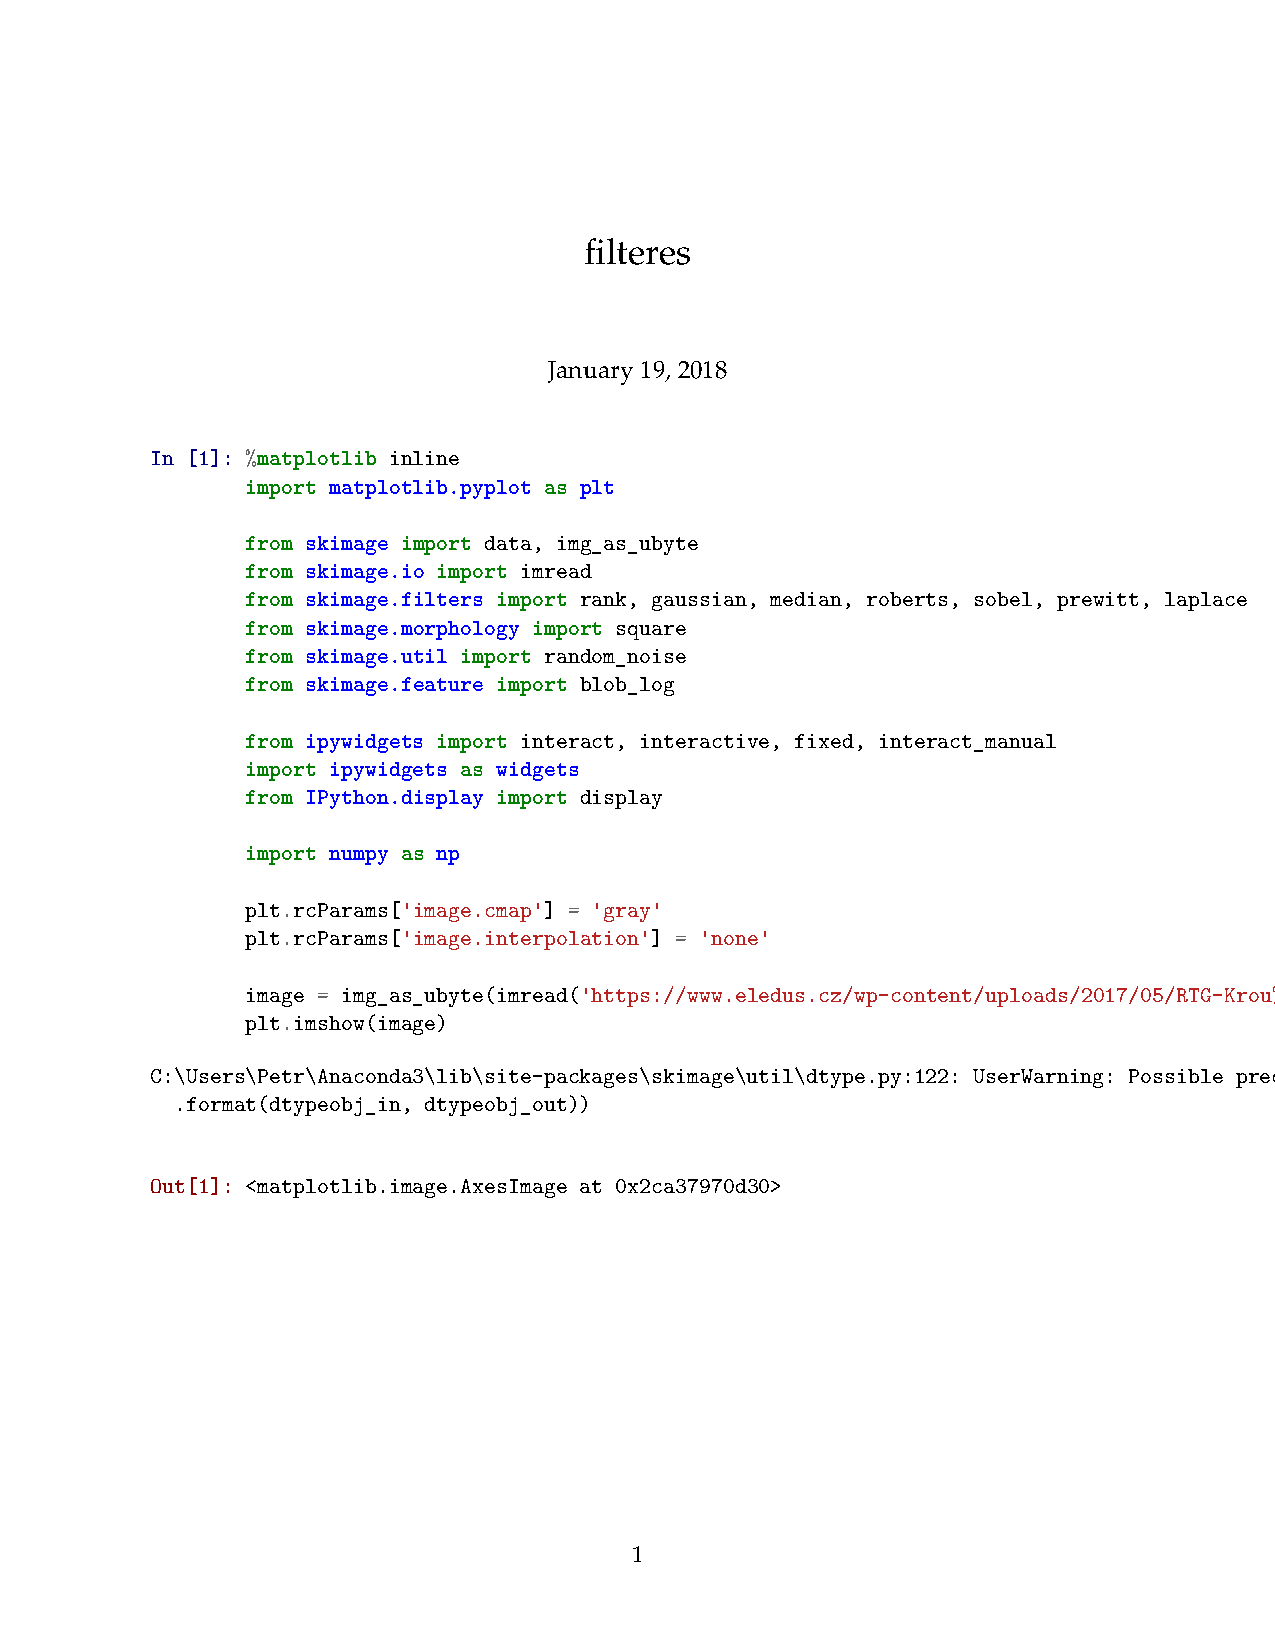
\includepdf[pages=-, scale=0.75]{pdf/current-methods-notebook.pdf}
\chapter{Implementace odstranění šumu průměrováním}
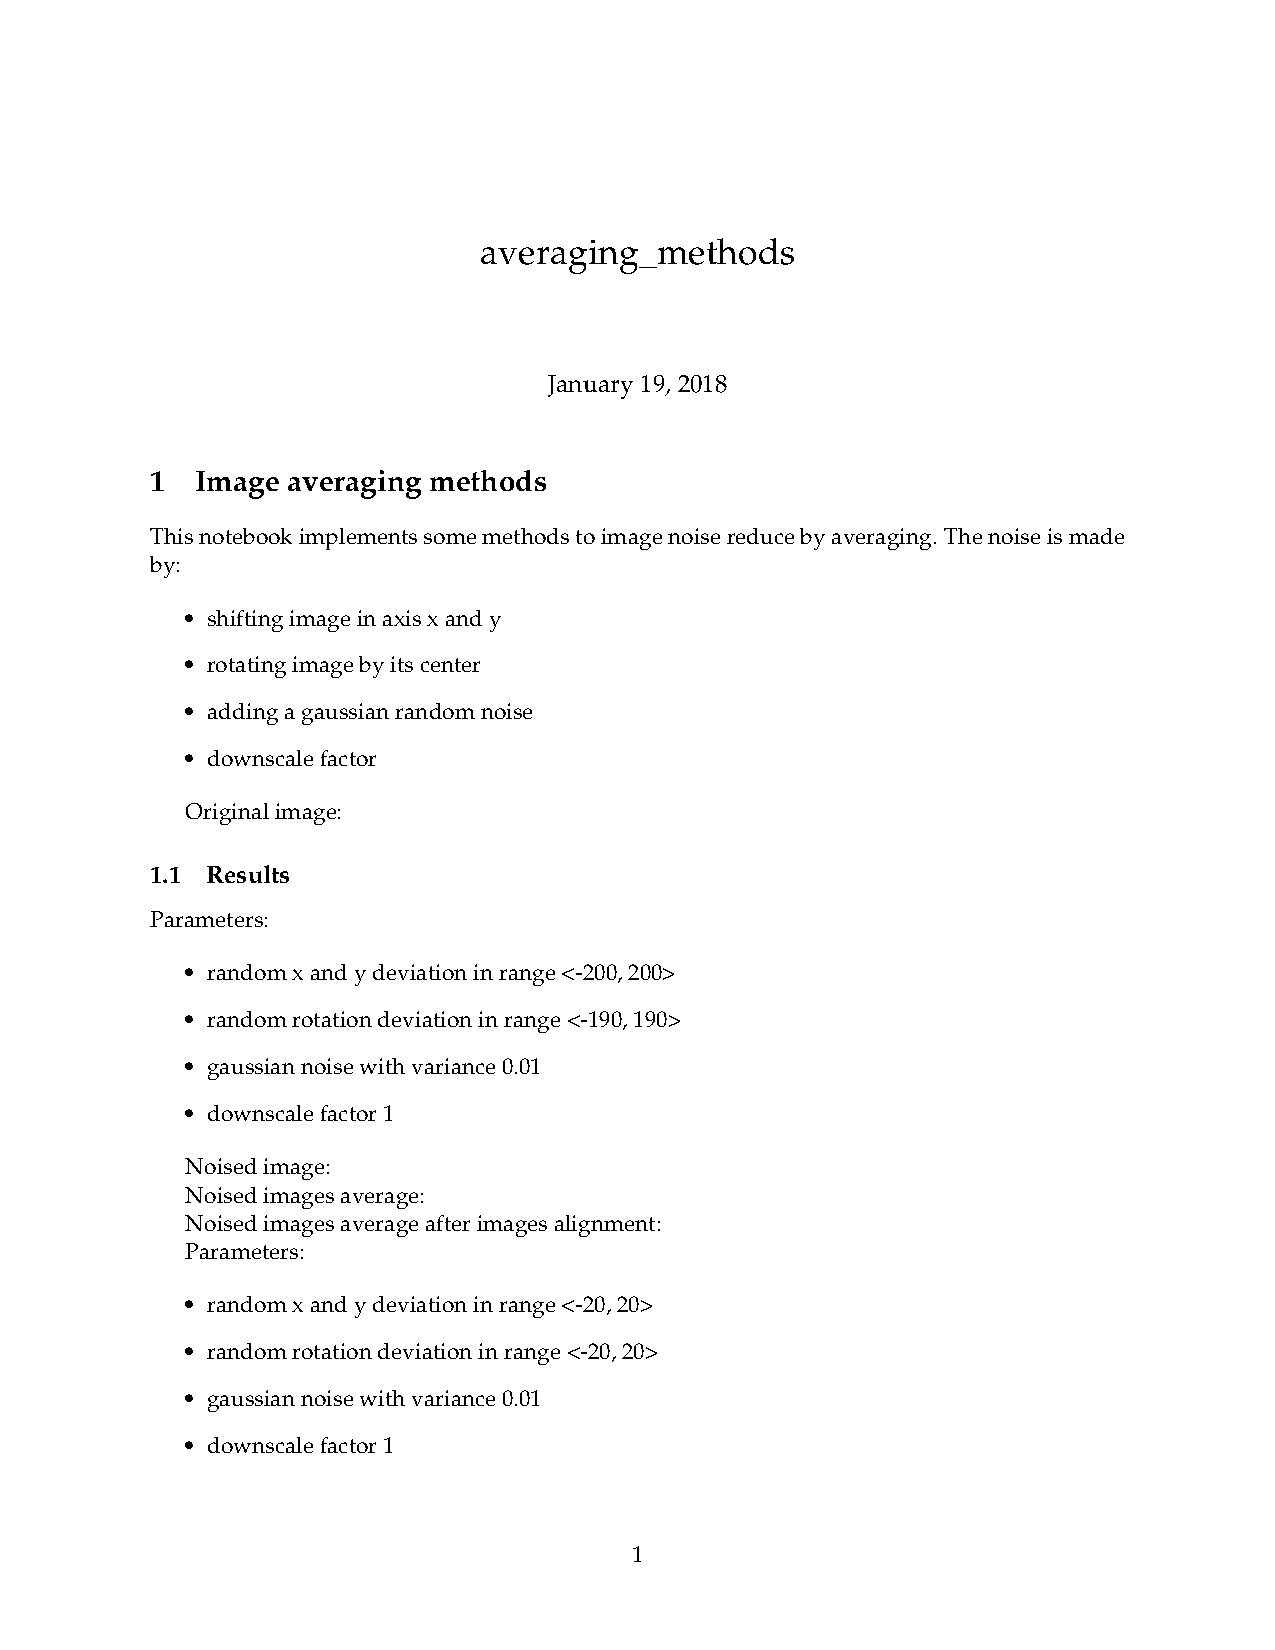
\includepdf[pages=-, scale=0.75]{pdf/averaging-methods-notebook.pdf}
\chapter{Implementace Debevec HDR}
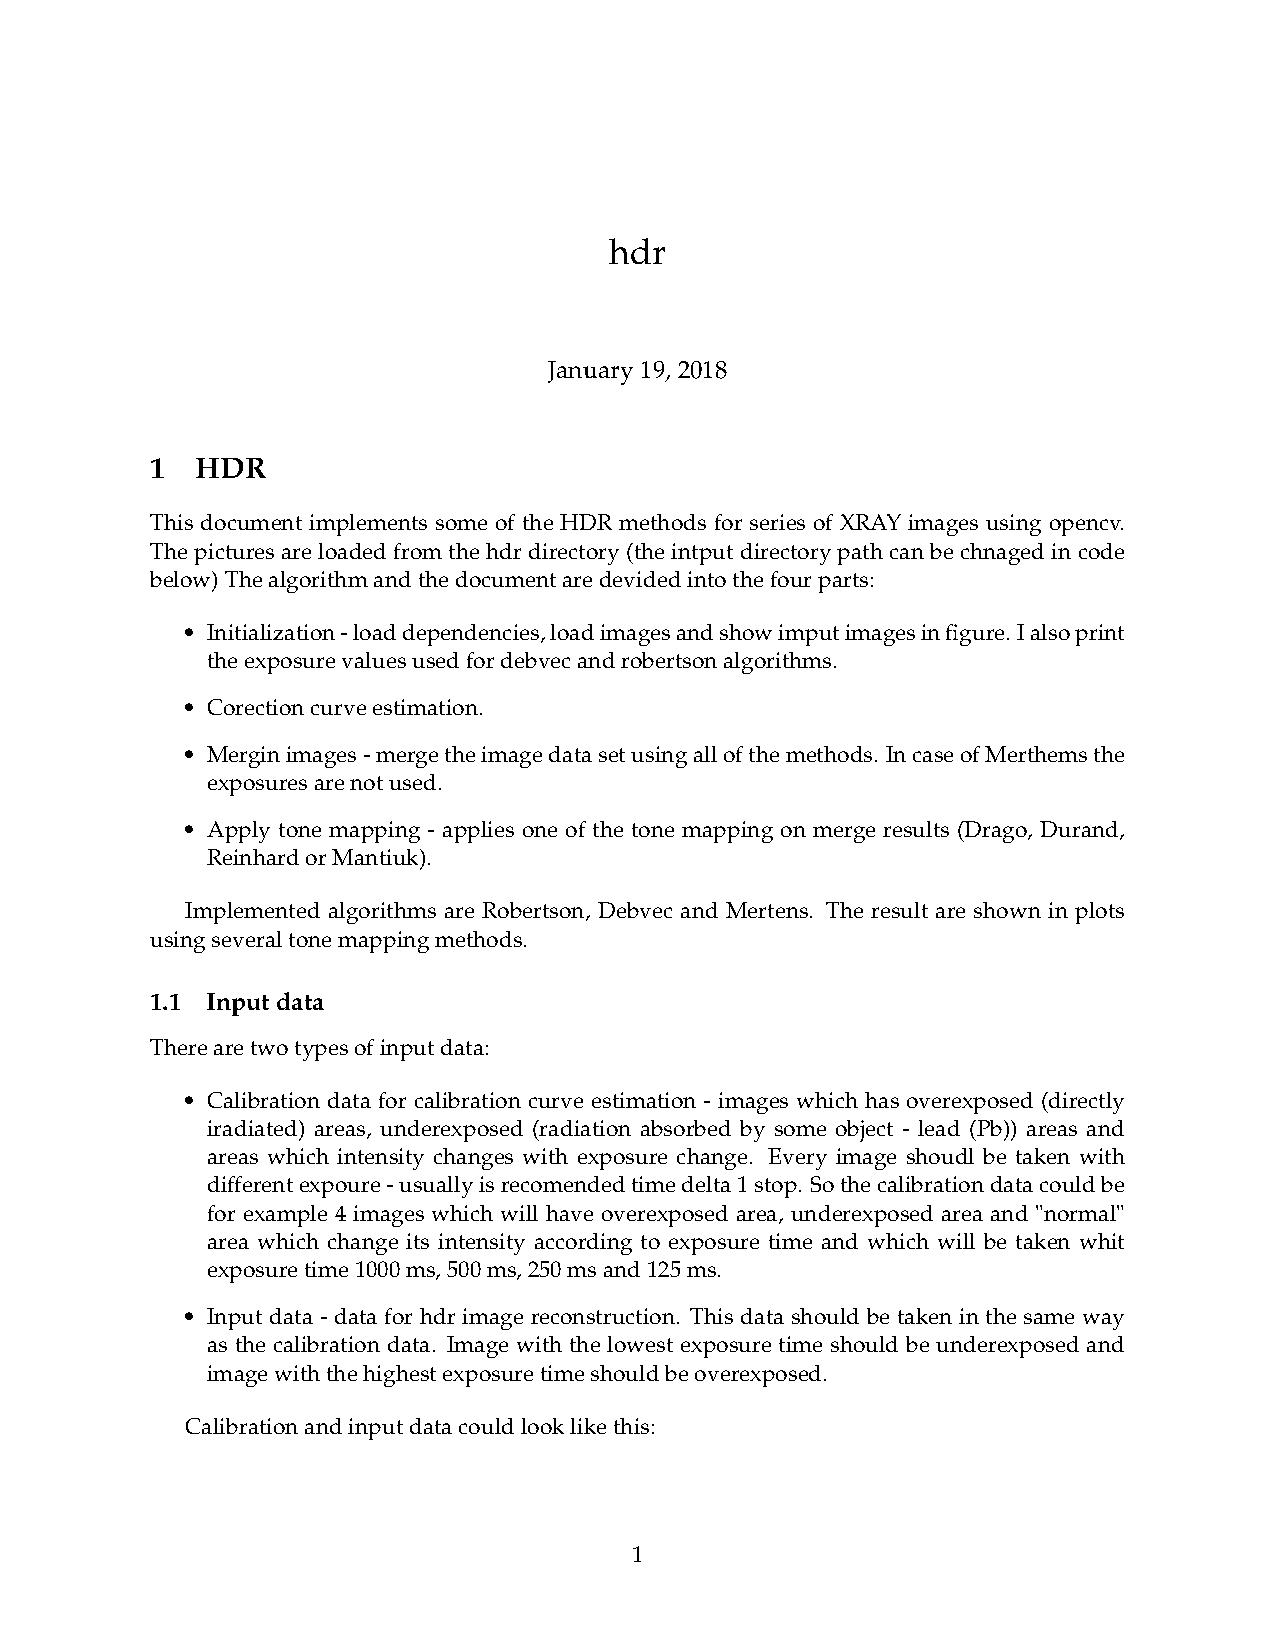
\includepdf[pages=-, scale=0.75]{pdf/hdr-notebook.pdf}
\shorthandon{-}